\chapter{Literature Review}\label{LitReview}

This research will focus on general purpose robots, operating in unstructured environments. More specifically it will focus on the grasping of dynamic objects. This section will outline existing research in grasping and grasping of dynamic objects. It will also explore related areas such as tactile servoing, robotic competitions, gripper design and more. It is through exploration of this prior research that the subject and direction of this project was informed.

\section{Existing Grippers}

There is a large and diverse range of existing robotic grippers, visible both in research and in industry. These grippers vary widely from simplistic to complex and from general purpose to having a very specific, niche applications. It would be difficult to complete a comprehensive review of all available grippers, however this section aims to introduce a subset, representative of the current state of the art. Inspired and expanding on the categories given by \cite{APCinhandproxandcontact}, grippers are discussed under the following headings and real world examples of each are given.


\begin{itemize}
    \item Pincer Grippers (Figures \ref{fig:YouBot}, \ref{label:Robotiq85} \& \ref{label:Hand-E})
    
    Pincer Grippers are one of the simplest types of gripper available. Despite their simplicity they are capable of a wide range of tasks. The result of low complexity and large application range is that they are one of the most used gripper morphologies. Pincer grippers use 2 opposing fingers to apply a clamping force onto the object. They require low control complexity but are inheriently limited and can encounter problems if the object is too large, heavy or irregularly shaped.
    
    \item Higher DOF  grippers (Figure \ref{lbel:Robotiq3Finger})
    
    These include robotic grippers with 3 or more fingers. Due to the larger number of fingers, and therefore DOF, the complexity, both mechanical and control, is higher. However, the number of grasp configurations which is possible also increases. These grippers have more potential as general purpose robotic grippers which could operate effectively in an unstructured environment, however due to their complexity they are more common in research than in industry. A comprehensive review of different types of grasp configurations is outside the scope of this document however has been explored in the literature previously \cite{GRASPTaxonomy}. The different finger configurations and associated grasps achievable with a 3-Fingered is explored by S. Tao, et. al \cite{Reconf3Finger}.
    
    
    \item Humanoid Grippers (Figures \ref{fig:Sandia}, \ref{fig:James}, \ref{fig:Allegro}, \& \ref{fig:DLR Hand II})
    
    Humanoid Gripper are in essence a subset of the "Higher DOF grippers" mentioned above but have the essential characteristic that they are similar to the human hand and are therefore worth considering in isolation. Gripper morphologies which are similar to that of a human hand tend to operate very well in unstructured environments \cite{pneumaticAnthropomorphicHand,Mahmoud2010}. 
    This can be attributed to the fact that the human hand is an excellent general purpose tool, but also because many of the unstructured environments which we wish robots to operate in tend to have been designed for easy of use by humans. They are therefore generally well suited to robotic grippers of a similar size, shape, degrees of freedom, etc. to a human hand. There other motivations to using a anthropomorphic gripper also. Their similarity aesthetically to a human hand makes them very desirable for prosthetics and they are desirable for applications where a gripper is tele-operated by a human since joint angles can be mapped directly from one to the other \cite{AnthroHandReview}. Similar to the previous category, the downside of these types of grippers is their complexity. The large number of fingers/DOF makes control difficult. They also tend to be very mechanically complex due to the large number of actuators required to control the large number of DOF.
    
    \item Vacuum Grippers
    
    Suction cup grippers are a common robotic end effector. A vacuum gripper uses a vacuum to adhere to the surface of the target object. Their usefullness is fundementally limited by the range of objects which they can manipulate. It is not possible to create a gripper which relies solely on a vacuum mechanism which can generalise to an arbitrary shape. This was particularly evident at the amazon picking challenge where teams struggled to pick up a variety of objects such as books, mesh cups, toilet brush, pencils, sponge, clothing and marbles when relying solely on a vacuum based gripper \cite{APCGripper, APCObservations}. Despite this they have proven very effective in certain applications and therefore very common in grasping applications. During the 2015 Amazon Picking Challange 36\% of the teams used some for of suction \cite{APCObservations}. They have proven popular in more structured environments where the object is consistent and an appropriate grasping target for a vacuum gripper. Since they are simple and effective for a large range of objects they are often implemented in a hybrid configuration with a more traditional gripper \cite{Nakamoto2019} to overcome some of their shortcomings. A vacuum-pincer hybrid gripper was identified as a suitable candidate to grasp in the cluttered narrow spaces presented for grippers used for warehouse automation \cite{Hasegawa2017}. Team Delft, winners of the 2016 Amazon Picking Challange, used a hybrid pincer and vacuum gripper\cite{Delft}.
    
    \item Other (Figures \ref{fig:Coffee Bean Gripper} \& \ref{fig:RBOHand2})
    
    There are more examples of types of grippers, typically for niche applications. These are outside the scope of this research but for the sake of completeness some will be mentioned here. The coffee bean gripper, seen in Fig. \ref{fig:Coffee Bean Gripper} uses a particle jamming mechanism to grasp objects. This technique is somewhat robust to different object geometries but struggles in some situations with grasp stability. The grasping procedure here is very simple, press the gripper on top of the object and activating the particle jamming by means of a vacuum pump to grasp the object. There is a reliance on the environment providing a reactant force when pressing on the object. Soft robotic grippers are also an active area of research \cite{RBOHand2}. These avoid using rigid components, substituting them instead for soft, passively compliant parts. These tend to be simpler to control, less expensive and inherently safe. However this typically comes at the cost of dexterity.
    
\end{itemize}

\begin{figure}
    \centering
    \begin{subfigure}{.3\linewidth}
        \centering
 %   
\includegraphics[width=.4\textwidth]{Images/placeholder.png}       
    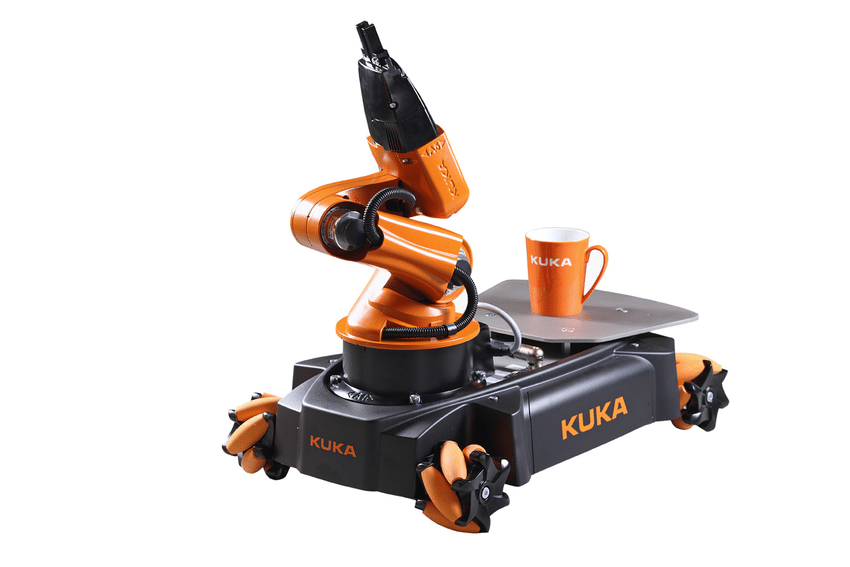
\includegraphics[width=0.7\textwidth]{Images/KukayouBot.png}
        \caption[youBot]{YouBot \cite{KukayouBot}}
        \label{fig:YouBot}
    \end{subfigure}
    \begin{subfigure}{.3\linewidth}
        \centering
        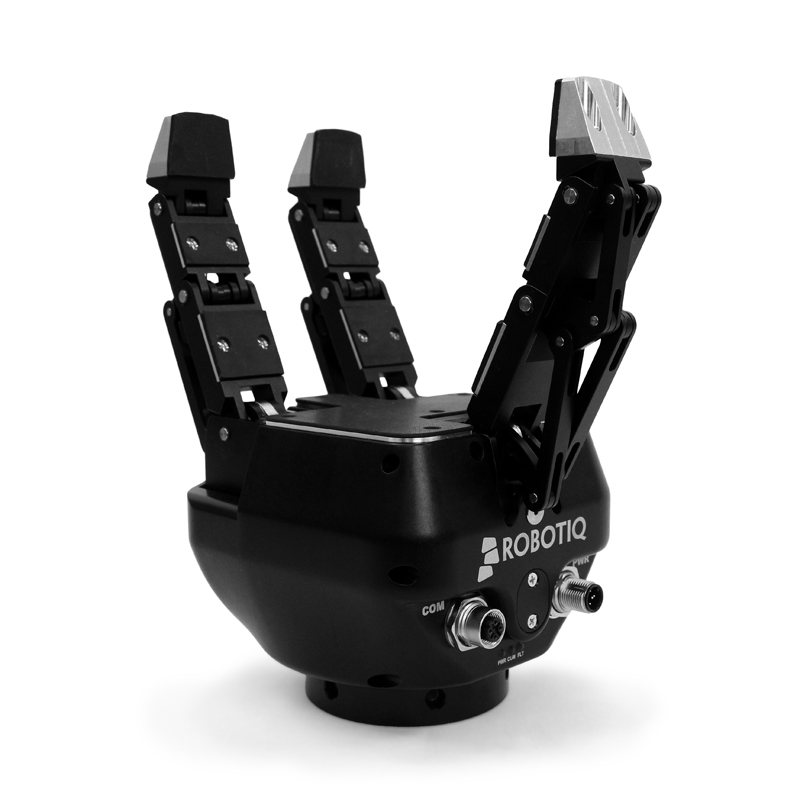
\includegraphics[width=0.7\textwidth]{Images/3-finger-robot-gripper-robotiq.jpg}
%    
\includegraphics[width=.4\textwidth]{Images/placeholder.png}
        \caption[3-Finger Adaptive Robot Gripper]{3-Finger Adaptive Robot Gripper \cite{RobotIQpic}}
        \label{lbel:Robotiq3Finger}
    \end{subfigure}
    \begin{subfigure}{.3\linewidth}
        \centering
%    
\includegraphics[width=.4\textwidth]{Images/placeholder.png}   
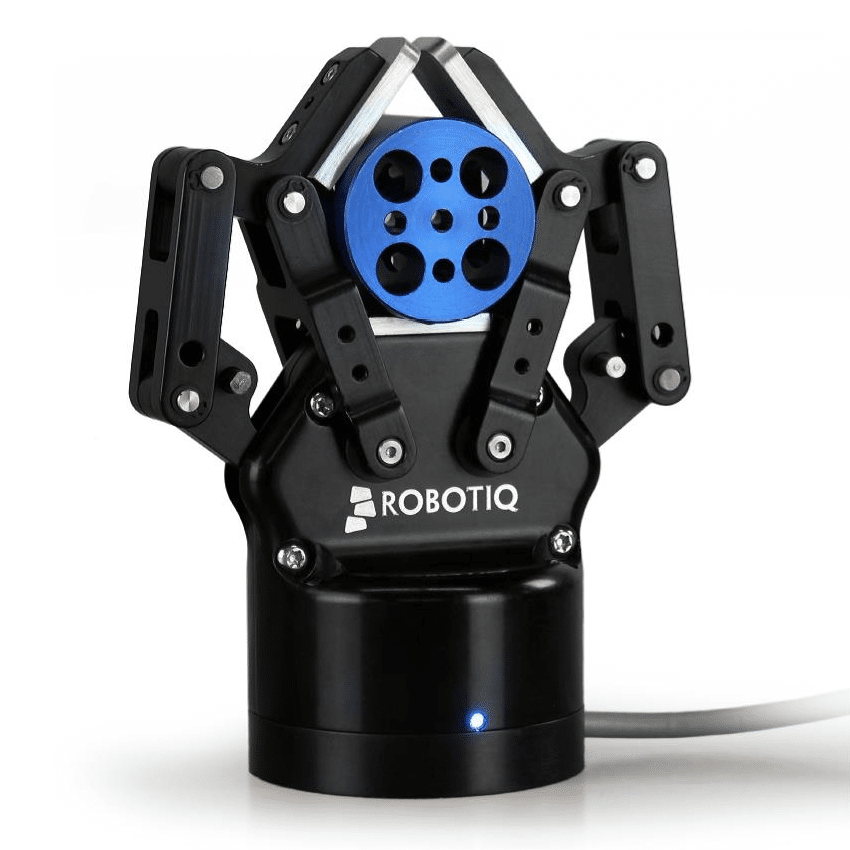
\includegraphics[width=0.7\textwidth]{Images/Robotiq-2-Finger-85-encompassing-grip.png}
        \caption[Robotiq 2F-85]{Robotiq 2F-85 \cite{RobotIQ2Fingerpic}}
        \label{label:Robotiq85}
    \end{subfigure}
    \begin{subfigure}{.3\linewidth}
        \centering
        \includegraphics[width=0.7\textwidth]{Images/Hand£.png}          
%    
\includegraphics[width=.4\textwidth]{Images/placeholder.png} 
        \caption[Robotiq Hand-E]{Robotiq Hand-E \cite{RobotIQHandEpic}}
        \label{label:Hand-E}
    \end{subfigure}
    \begin{subfigure}{.3\linewidth}
        \centering
        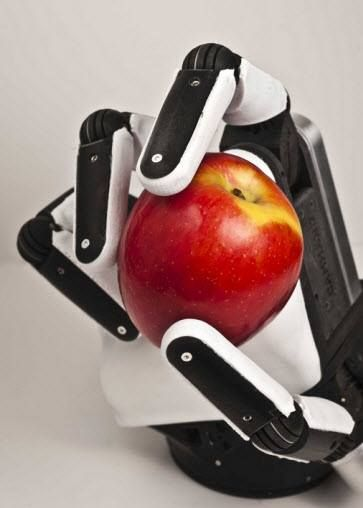
\includegraphics[width=0.7\textwidth]{Images/Sandia.jpg}       
  %  
\includegraphics[width=.4\textwidth]{Images/placeholder.png}
        \caption[Sandia Hand]{Sandia Hand \cite{SandiaHand}}
        \label{fig:Sandia}
    \end{subfigure}
    \begin{subfigure}{.3\linewidth}
        \centering
        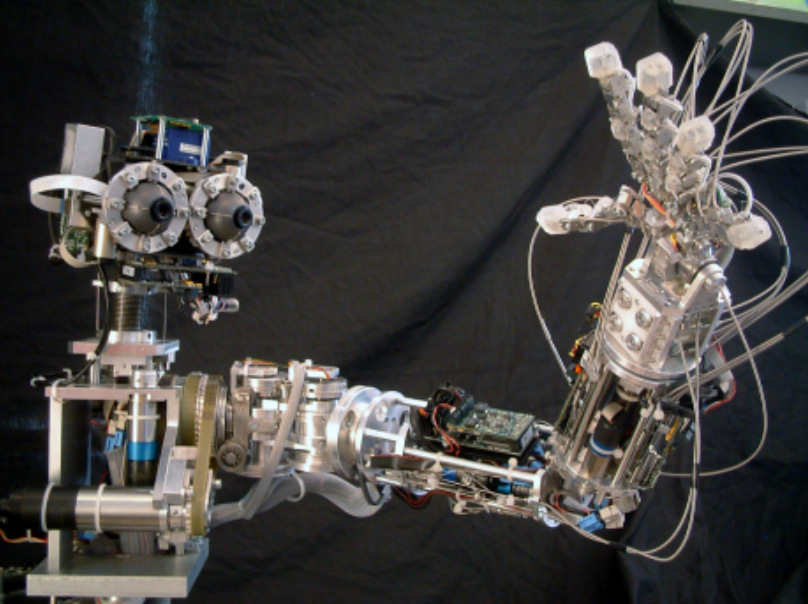
\includegraphics[width=0.7\textwidth]{Images/James.png}    
  %  
\includegraphics[width=.4\textwidth]{Images/placeholder.png}
        \caption[James]{James \cite{James}}
        \label{fig:James}
    \end{subfigure}
    \begin{subfigure}{.3\linewidth}
        \centering
        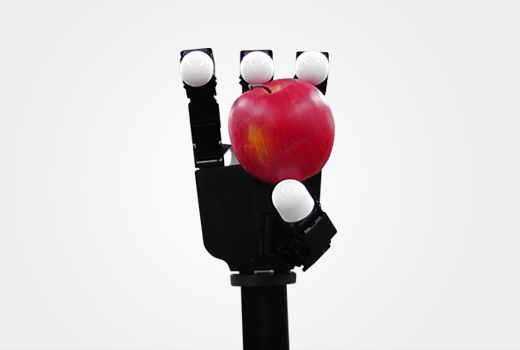
\includegraphics[width=0.7\textwidth]{Images/Allegro_Hand_flash_03.png}
 %   
\includegraphics[width=.4\textwidth]{Images/placeholder.png}
        \caption[Allegro Hand]{Allegro Hand \cite{AllegroHandpic}}
        \label{fig:Allegro}
    \end{subfigure}
    \begin{subfigure}{.3\linewidth}
        \centering
        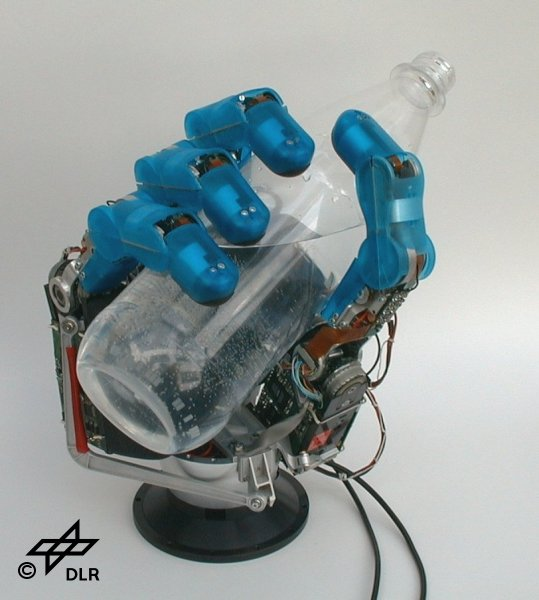
\includegraphics[width=0.7\textwidth]{Images/Hand-II-01.jpg}   
  %  
\includegraphics[width=.4\textwidth]{Images/placeholder.png}
        \caption[DLR Hand II]{DLR Hand II \cite{DLRHandIIpic}}
        \label{fig:DLR Hand II}
    \end{subfigure}
    \begin{subfigure}{.3\linewidth}
        \centering
      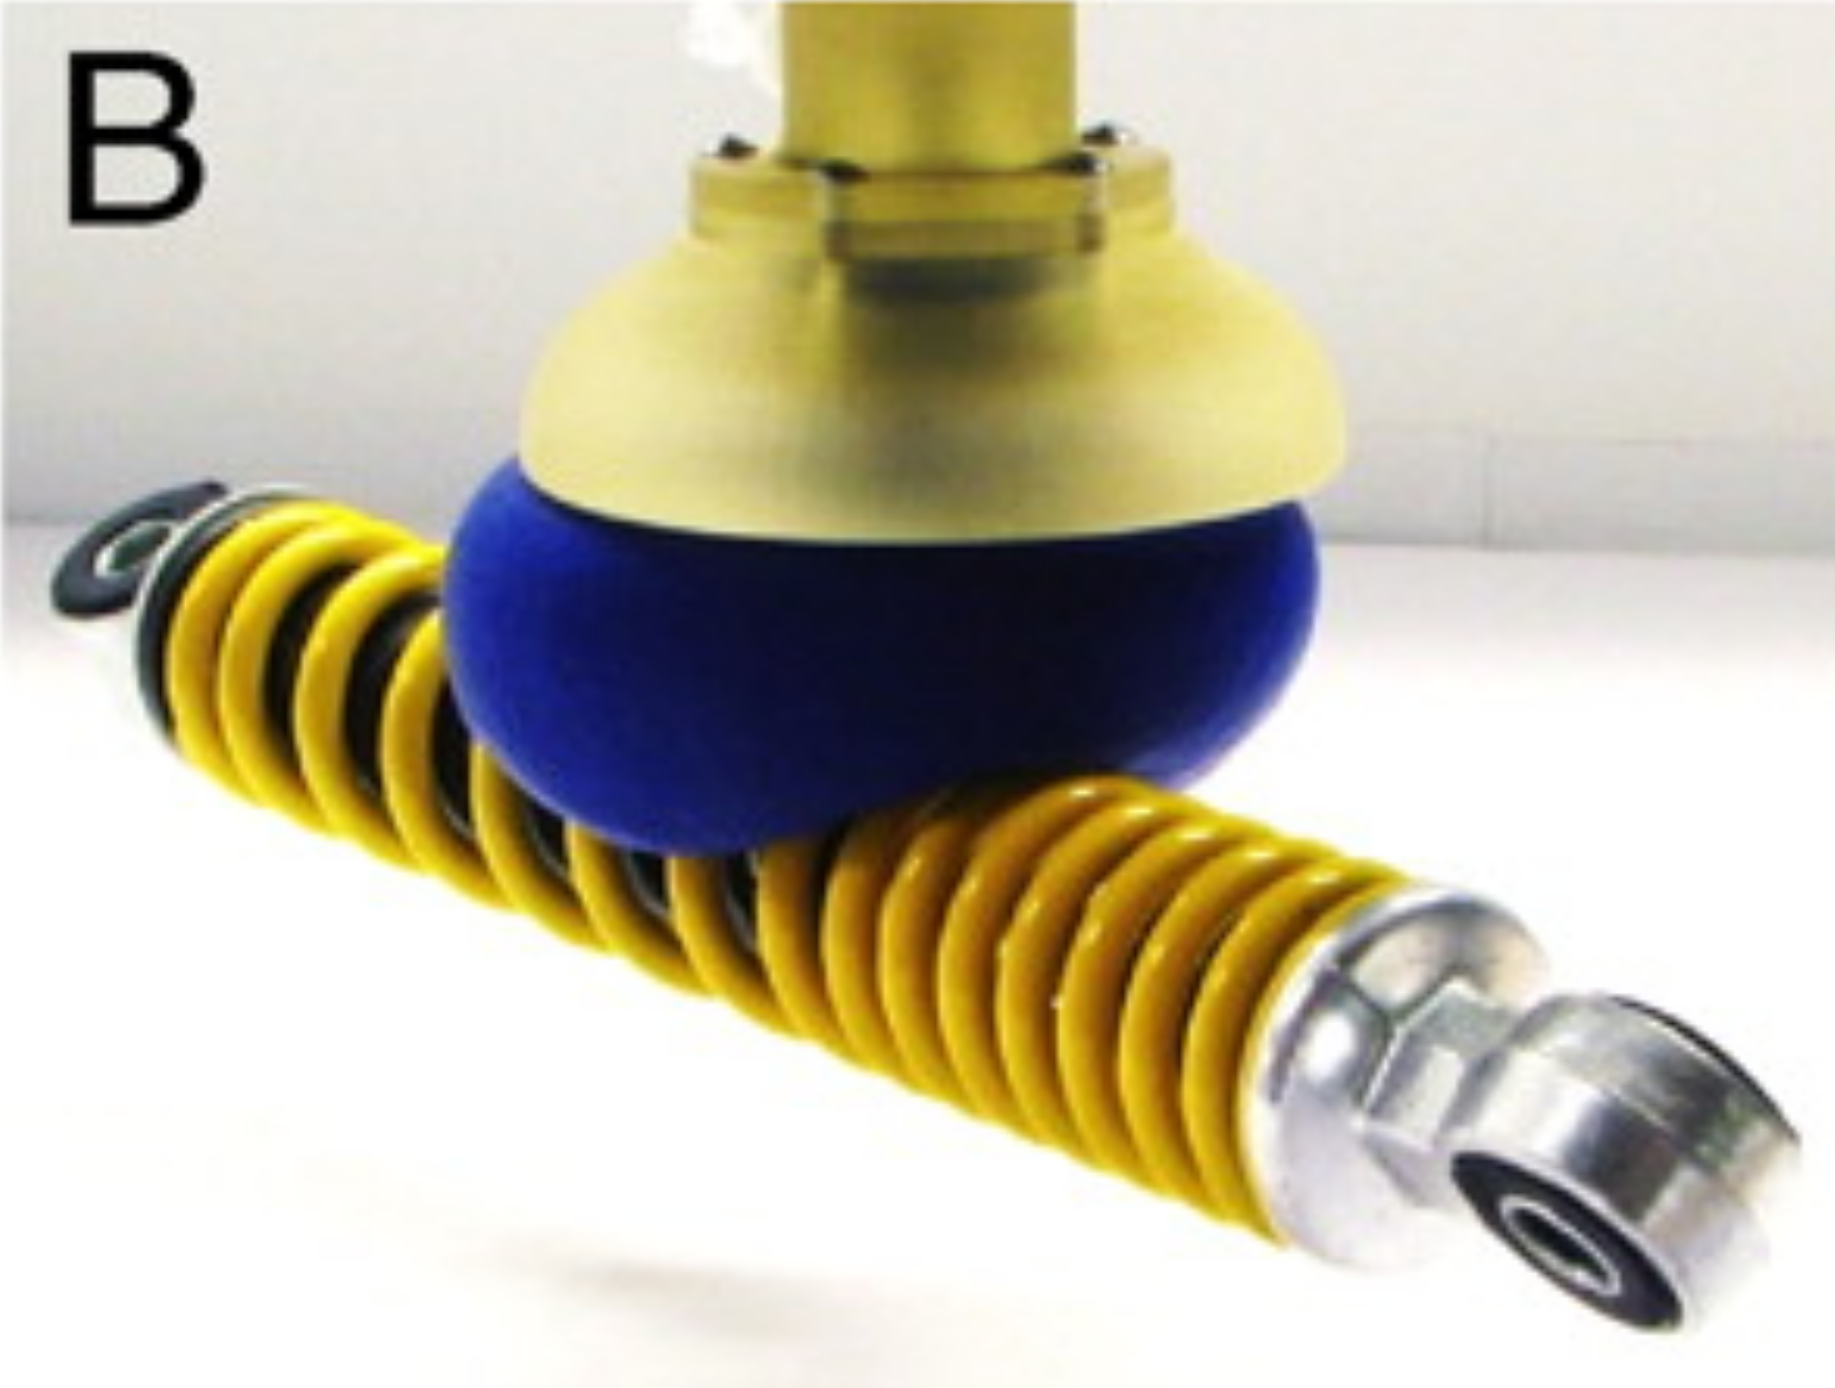
\includegraphics[width=0.7\textwidth]{Images/CoffeeBeanGripper.png}   
  %  
\includegraphics[width=.4\textwidth]{Images/placeholder.png}
        \caption[Coffee Bean Gripper]{Coffee Bean Gripper \cite{ParticleJamming}}
        \label{fig:Coffee Bean Gripper}
    \end{subfigure}
    \begin{subfigure}{.3\linewidth}
        \centering
    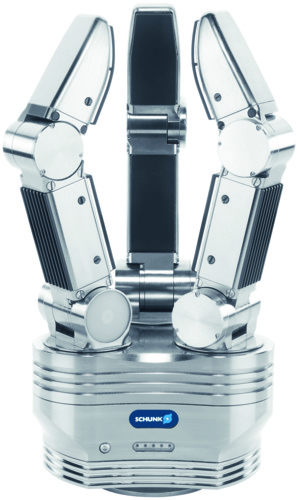
\includegraphics[width=0.7\textwidth]{Images/Schunk3FingeredGripper.jpg}
%         
\includegraphics[width=.4\textwidth]{Images/placeholder.png}
        \caption[Schunk 3 Fingered Gripper]{Schunk 3 Fingered Gripper \cite{Schunk3FingerGripper}}
        \label{fig:Schunk3FingeredGripper}
    \end{subfigure}
    \begin{subfigure}{.3\linewidth}
        \centering
        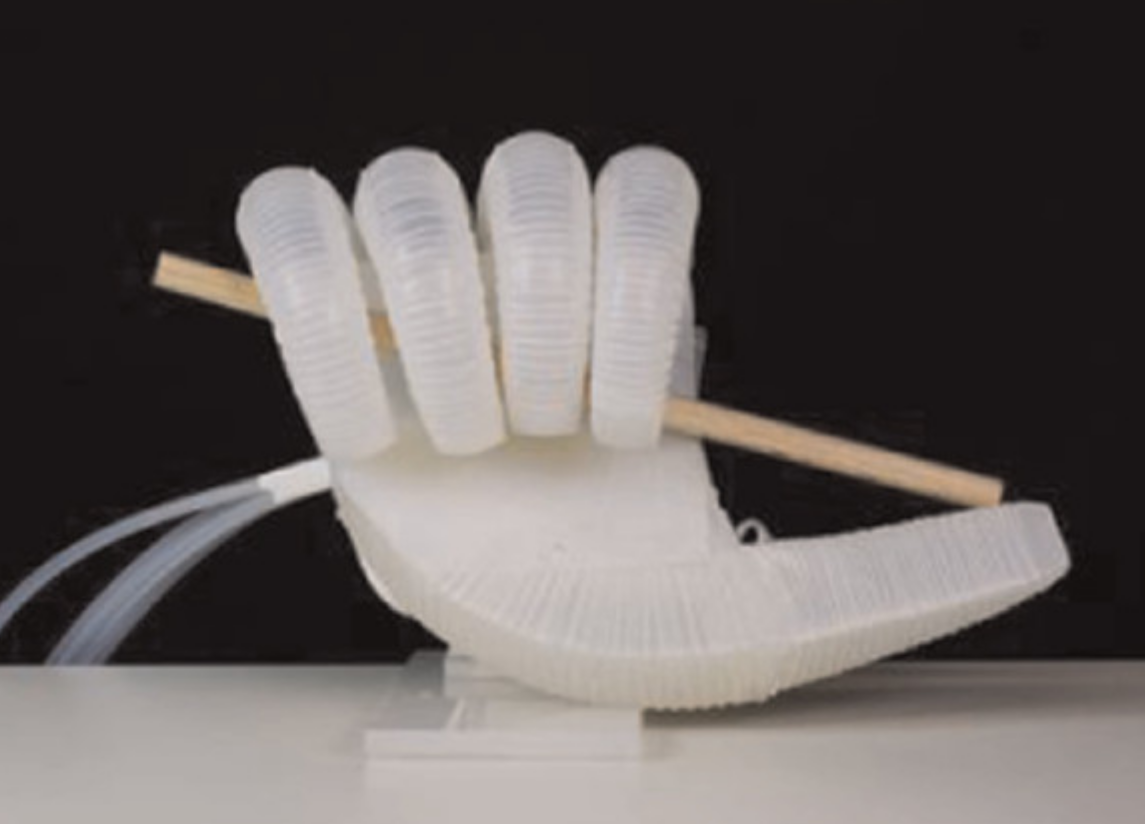
\includegraphics[width=0.7\textwidth]{Images/SoftRoboticGripper.png}
    %     
\includegraphics[width=.4\textwidth]{Images/placeholder.png}
        \caption[RBO Hand 2]{RBO Hand 2 \cite{RBOHand2}}
        \label{fig:RBOHand2}
    \end{subfigure}
    \caption{Selection of existing grippers}
\end{figure}

\section{Grasp Sensing}
Sensing is a vital part of any gripper and grasping motion. Without sensing, only highly structured tasks can be achieved. Sensing can typically be divided into two types, proprioceptive sensing and exteroceptive sensing. The former describes sensing which is used to measure physical information related to the current state of the system, i.e. joint angles, velocity, etc. This is critical to ensure that the robot behaviour is as expected, i.e. to use closed loop control. The latter refers to sensors which offer information about the target object or environment, i.e. force, pressure, temperature, etc. Exteroceptive sensing offers the ability to adapt to changes in its environment, to infer information about the object and environment and inform the actuation accordingly. Sensing is a fundamental building block of any general purpose gripping system. This section will examine some of the most common and most relevant types of sensing to grasping moving objects. 

\subsection{Image Sensing}

Autonomous robotic grasping and has always relied heavily on image sensors to provide the information needed to grasp the target object. Image sensing, both 2D and 3D, has many advantages over other types of sensing. It provides high resolution sensor data which can be collected in a non-intrusive way. Information about the object can be collected without physical interaction with the target object. For these reasons it has become the primary sensing mode used in manipulation and grasping tasks. Examples of the use of image sensors in grasping applications are present both in robotics research, and commercial products. The RobotIQ, pincer gripper with built-in image sensing shown in Figure \ref{fig:RobotIQImageSensing} is just one of example in a comercial context. Furthermore, all examples of grasping moving objects examined later in this chapter use image sensing in some capacity. This is particularly evident when examining robotics competitions, for example all robots participating in the 2015 Amazon Picking Challenge (APC)\cite{APCObservations} used image sensing. The use of image sensing in the 2015 APC is summarised in table \ref{table:APCSensorBreakdown}.

There are also difficulties associated with the use of image sensing. This type of sensing collects vast quantities of data, much of which is not relevant. Large amounts of computational power is required to filter and analyse the collected data to extract useful information. This becomes an important factor when grasping moving objects since the task is time critical. It is also a concern on robotic platforms which are computationally limited such as mobile platforms.

Robotic image sensing can generally be split into two distinct categories, 2 Dimensional (2D) and 3 Dimensional (3D) image sensing. Each is named for the type of data which it collects, ie. 2D image sensing refers to sensors which collect a 2D photograph of the scene whereas 3D image sensing collect 3D data about the environment, such the depth of an object, or the distant to a point. There is several ways in which depth information can be collected. The two most common are stereo camera pairs and depth cameras. Stereo pairs operate using the same mechanism as the human eyes. A pair of traditional 2D image sensors are placed a know distance apart. Using difference between the two images collected and basic geometric calculations, depth information can be inferred. Depth cameras use a different mechanism, they project IR light patterns of a known structure onto the environment and extract depth information from how the patterns interfere with the scene. This mechanism is used in commercial depth cameras like the Microsoft Kinnect and Asus Xtion \cite{APCinhandproxandcontact}.

IR image sensing is a less commonly used form of image sensing. That being said, it is incredibly useful in certain applications. IR sensing is similar to traditional 2D image sensing with the exception that the sensor is sensitive to IR light rather than the visible spectrum. For this reason it can be very useful for interacting with humans since humans emit IR radiation allowing easy segmentation from their surroundings \cite{HumanIR}. IR image sensing is also used in manipulation, often for niche applications such as sorting and grading fruit based on ripeness \cite{MangoTest}, or assessing the integrity of power lines \cite{IRPowerLines}. One final use of IR image sensing in robotic manipulation is the use of IR reflectors as markers to simplify localisation. An example of this is the OptiTrack system \cite{OptiTrack} used by Seungsu Kim, et. al. to facilitate the grasping of tennis rackets and water bottle which are tossed at the robot \cite{TennisRacket}. These reflectors can be seen as silver spheres on the tennis racket in figure \ref{fig:IRMarkers}.

\begin{figure}
    \centering
    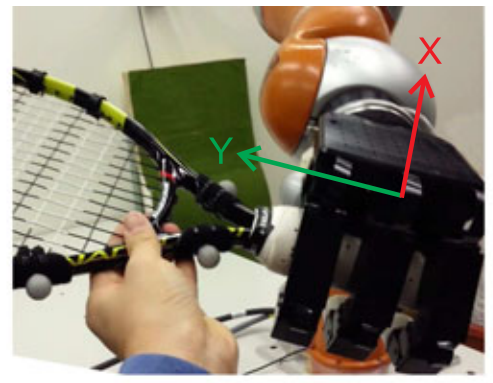
\includegraphics[width=.4\textwidth]{Images/CatchingObjectInFlight.png}
   % 
\includegraphics[width=.4\textwidth]{Images/placeholder.png}
    \caption{Dobot M1, soring and orientating chewing gum}
    \label{fig:IRMarkers}
\end{figure}

\begin{figure}
    \centering
       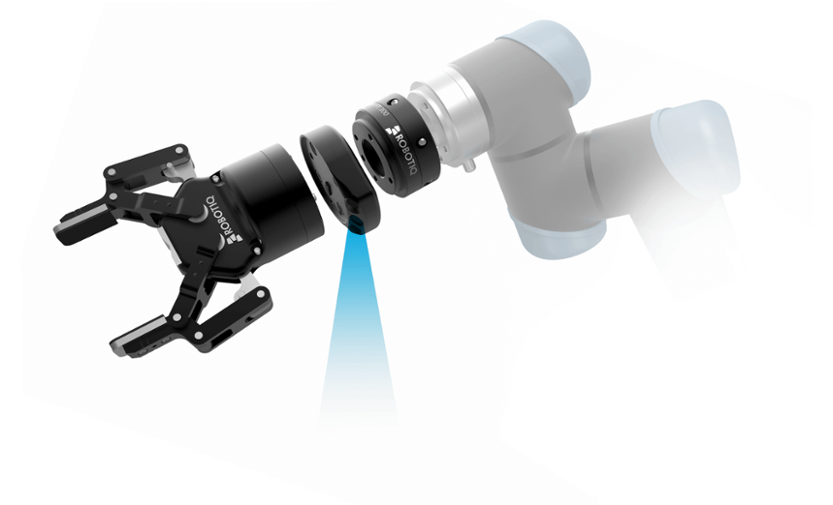
\includegraphics[width=0.4\textwidth]{Images/robotiq-vision-guided-robotic-hand-system.png}
%    
\includegraphics[width=.4\textwidth]{Images/placeholder.png}
    \caption[RobotIQ hand using image sensing]{RobotIQ hand using image sensing \cite{RobotIQVisionPic}}
    \label{fig:RobotIQImageSensing}
\end{figure}

\begin{table}[ht]
\centering
\begin{tabular}{|l|l|l|l|l|l|}
            & Head & Torso & End-effector & Arm & Total respondents\\  \hline
2D imaging  & 4    & 1     & 4            & 1   & 20 \\  
3D imaging  & 8    & 3     & 6            & 6  & 7  
\end{tabular}
\caption[Use of Image Sensing in the 2018 Amazon Picking Challenge]{Use of Image Sensing in the 2018 Amazon Picking Challenge, excerpt from \label{table:APCSensorBreakdown}
\cite{APCObservations}}
\end{table}

% Tactile Sensing
\subsection{Tactile Sensing}

Tactile sensing is a core component of how humans interact with and explore their environment. Experiments have shown how the loss of a ``sense of touch" is detrimental to a human's ability to grasp and manipulate objects \cite{HumanTactile}. Roboticists have long thought that endowing a robot with a ``sense of touch" would be beneficial, and perhaps necessary, to enable them to interact with an unstructured world \cite{iCub}. 

Tactile sensing is commonly used to detect collisions or contact points \cite{ConveyorBelt}. It can also be useful for understanding the nature of objects; it can help a system infer information about an object's properties like size, shape, weight, texture and temperature \cite{ObjectExploration,Vizzy,uSkinFingertip,InHandCP, TactileMango}, and can also be used to detect slip and shear between gripper and object \cite{First3DHall,HumanstoHumanoids,Survey}. It is therefore useful in object exploration \cite{TSiCub,BimanualExploration}, object classification \cite{James}, in-hand manipulation \cite{InHandCP} and grasping tasks \cite{Gifu}. 

Tactile servoing is one particularly relevant area of research were tactile sensing is used. Tactile sensing being used to inform and control the motion of a robotic gripper referred to as tactile servoing. The initial concept for tactile servoing proposes that the progress of a manipulation task can be observed and monitored through the sensor data from embedded tactile sensors in the gripper \cite{1994TS}. In recent years, tactile servoing has expanded and successfully enabled researchers to achieve tasks such as active contour following, object shape construction and object manipulation \cite{TSiCub,ContactControl}. Although tactile servoing research has shown potential to improve robotic grasping, research has encountered several problems. Imperfections in tactile sensing arrays \cite{TSdexterous}, noisy sensors \cite{1994TS}, computationally expensive models \cite{ContactControl}, and poor data interpretation \cite{Overview} are frequently reported in the literature.  Therefore, despite many examples of the use of tactile sensors to contribute to the control of a gripper grasping static objects, the potential contribution of tactile sensing towards grasping a moving object is still an under-explored research area.

Prior research has examined the nature of tactile sensing in more detail and rigorously categorised different types \cite{HumanstoHumanoids,TSdexterous}. For the purpose of this report we will summarise some of the commonly used types, and examine the advantages and disadvantages of different approaches. We will use the sensing mechanisms to categorise different approaches.


\begin{itemize}
    \item Hall Effect
    
    Tactile sensing based on the hall effect utilises a magnetic field to determine information about contact with an object. Typically in a hall effect based tactile sensor the position of a magnet relative to a hall effect sensor (a sensor which can measure the strength of a magnetic field) is in some way related to the current state of contact between the robot and an object. Therefore, details about the nature of contact , i.e. location, pressure, etc. can be inferred from reading the strength of the magnetic field. There are many example of such sensors in the literature, a recent example of this is uSkin \cite{uSkinFingertip} which has been applied and used in research to grippers such as the Allegro hand \cite{Allegro} and the iCub gripper \cite{iCub}
    \item Capactive
    
    Capactive tactile sensing uses the physical phenominium that the potential different between 2 conductors, separated by an insulator, is dependant on the distance between them. Using this, tactile sensors can use a soft, elastic material to act as the insulator between 2 conductors. In this way the capacitance will reflect the deformation of the elastic insulator and allow the robot to infer information about nature of contact with an object. 
    \item Pressure
    
    Pressure based tactile sensors also rely on an easily deformable, elastic material. In this case a pressure sensor (barometer) measures the pressure of the material. This pressure will respond in a predictable way to contact forces on the material, representing contact between the robot and an object.
\end{itemize}




\subsection{Joint Feedback}
Joint Feedback is an example of proprioceptive sensing, enabling the robot to monitor the position of each of its joints and therefore extrapolate its own position in space. This type of sensing is essential for control purposes, i.e. to provide feedback to the motor controller to ensure that the desired motion is achieved. There are many different mechanisms which can be used to provide joint feedback , these are discussed below.
\begin{itemize}
    \item Magnetic Encoders
    
    Magnet encoders also rely on the hall effect, and are used to monitor the position of a shaft. The relative orientation of two parts of the robotic system is monitored by attaching a magnet to one and a hall effect sensor to the other. The magnetic field measured is dependant on their relative orientations and the position of the joint can therefore be inferred.
    \item Optical Encoders
    
    Optical encoders measure relative rotation between two parts of a robotic system. Unlike magnetic encoderes they do not measure in absolute terms but monitor the relative movement of a shaft. A disc with a pattern of slits in attached to the rotating shaft, an IR emitter-receiver pair is attached to the parent robot. The emitter is placed on 1 side of the disc and receiver placed on the other. The pattern of flashes, detected by the receiver when the slit aligns with the emitter, can be analysised to give information about the rotation. 
    \item Mechanical Encoders
    
    Mechanical encoders use a similar mechanism as optical encodes and attach a disc with a custom pattern to the rotating shaft. In this case it is mechanical contacts which interacts with the disc and produce an electrical signature representative of the movement of the shaft.
    \item Potentiometer
    
    Finally, potentiometers or variable resistors can be used to sense joint position. The potentiometer used in this application generally has a resistance determined by the relative orientation of an internal shaft to the rest of the sensor. By coupling this internal shaft to a joint shaft the joint angle can be measured. A draw back of this type of joint sensor is that the variable resistor will have some maximum and minimum resistance which it can achieve and is therefore unsuitable for measuring contineous rotation. In reality potentiometers either have a finite angle of rotation or have a discontinuity in their resistance at some angle. This is generally not a problem for robotic gripper or manipulator joints which also tend to have a finite joint angle range and don't require contineous rotation.
\end{itemize}

\subsection{Misc Sensors}

There a huge number of sensors which have previously been implemented in robotic systems, however it is outside the scope of this document to complete a full review. There are some other, less common, examples which are particularly relevant to this research and so will be mentioned here. Although depth cameras have been mentioned, there are a range of other types of range finding sensors, i.e. time-of-flight light sensors, LIDAR and ultrasonic sensors, which are common in robotic gripper systems. A more niche example is the work of Ilhan Konukseven et. al. \cite{FingertipEmitterReceiverMovingObjectII, FingertipEmitterReceiverMovingObject}. In this research a custom sensor is developed to calculate an error in alignment between the axis of the gripper and the axis of symmetry of the object to aid in grasp alignment. Whisker-like sensors, inspired by whiskers on animals, have also been explored in robotics as a way of exploring unknown environments \cite{2000Konukseven}. The use of whisker sensors have been explored on wheeled robots for close wall following \cite{CloseWallFollowing} and in manipulation for object localisation, recognition and grasping \cite{TactilePerception}.


\section{Actuation}\label{Actuation}
Actuation is a fundamental part of any manipulation system, actuators are the components which enable a system to move. At a very high level the actuator will take some energy input, usually in the form of electrical or potential energy and convert it to kinetic energy. In the manipulation context, actuators are essential both for moving the end effector into position and to enable the end effector to grasp the object. This research is most concerned with the motion which grasps the object however similar actuators are used in all areas of robotics. This section will look at the most common actuators used in robotic grippers to date, the advantages and disadvantages, the trade-offs and the applications. This section will also examine actuation strategies and the advantages and disadvantages of underactuated systems compared to fully actuated systems.

The first method of actuation discussed is the DC motor. A simple system where an electric potential input will cause a shaft to rotate. They are effective in a large range of sizes. They are inexpensive and efficient, making them the most commonly used method of actuating any part of a robot. Despite this there are several disadvantages. DC motor produce maximum power and are most efficient at high speeds, this results in the use of gears and other motion transmission methods which reduce the speed while increasing the torque. Although this trade off, more torque for less speed, is advantageous for robotic applications there are inefficiencies and errors associated with these devices. Friction, noise and backlash are all problems which are introduced while making the system more expensive. Backlash in particular is a problem for robotic manipulation. In order to maximize the number of poses which the manipulator can position and orientate its end effector in, a manipulator generally has a large number of Degrees of Freedom (DOF). Similarly to maximise the flexibility of a gripper it also has a large number of DOF. In both cases these DOF are arranged in a relatively long, open kinematic chain. The effect that blacklash and any other error between the desired and actual joint angle is that these errors propagate and accumulate through the chain such that small relative errors caused by backlash at each joint causes a large absolute error in the position of the end effector.

%% Potentially a nice Diagram of error propagation

A further disadvantage of using simple DC motors is the absence of a feedback mechanism. The speed of a DC motor is largely determined by the voltage applied and the output torque is proportional to the current. Due to variations in these parameters and the effects of a load on the shaft it is difficult to determine the position of the motor at any particular time, based on the inputs to the motor. Furthermore using the inputs to a DC motor as a way of determining the position of a robot joint is subject to error propagation since the voltage input determines speed and in robotic manipulation we are generally interested in joint position. For example a small error in the estimation of the motor speed would cause an ever growing error in the joint position over time. For this reason, simple DC motors are almost always implemented with an separate feedback mechanism.

Stepper Motors are another common method of actuation in robotics and one which addresses this problem. They are similar in some ways to a simple DC motor but overcome some of the challenges while introducing its own challenges. Like a simple DC motor a stepper motor takes DC electricity as an input and produces kinetic energy in the form of a rotating shaft. The internal differences between a simple DC motor and a stepper motor are outside the scope of this document but in effect the mechanism by which a stepper motor operates allows position controlled unlike a speed controlled simple DC motor. This ability to control the position of the motor comes at the cost of requiring logic to control the motor, generally in the form of a micro-controller. Steppers motors also exhibit holding torque, a feature which other DC motors lack. A stepper motor can hold its shaft in position opposing external forces. This is often useful in manipulation applications.

Motors are the most common form of actuation in robotics, and the form using in this project however other types of actuation include piezo electrics, pneumatics and hydraulics. Each with its own set of advantages and drawbacks. These will not be discussed in this document.

\subsection{Under Actuation}\label{UnderActuaction}

Underactuation is a technique often used in robotics, among the mostly commonly cited reasons for choosing to underactuate a system is to reduce the number of actuators required \cite{UnderactuationReductionInActuactors}, to simplify the control and therefore computational overhead and to fully take advantage of the system's natural dynamic characteristics \cite{PassiveDynamicWalker}. A system is said to be underactuated if the number of dimensions in which it is free to move, i.e. its Degrees of Freedom (DOF) is more than the number of independently actuated joints. Most robots can be described by 

\begin{equation}
\ddot{q} = f_1(q,\dot{q},t) + f_2(q, \dot{q},t)u   
\end{equation}
where \(u\) is the control vector, \(t\) is time and the robot's state can be described by a vector of positions (\(q\)) and velocities(\(\dot{q}\)). If 
\begin{equation}
    rank[f_2(q,\dot{q},t)] < dim[q]
\end{equation}
then the system is said to be underactuated.

More specific to robotic grippers, underactuation can often be a desirable quality and give the grasper the ability to self-adapt to object geometry. One way to achieve this is through use of elastic or flexible material to mechanically couple joints in the finger. This allows the gripper to better adapt to the shape of an object and increase the chances of a successful grasp simply by carefully designing and utilising the physical embodiment of the hand.

However it has been found that underactuation tends to hinder grasper dexterity \cite{RBOHand2}. Using this method inheriently, forfeits independent control over each joint individually. That being said, through tuning the moments and elastic elements at each joint the order in which the joints act, when the finger is actuated, can be controlled. The most common use of this, shown in figure \ref{UnderActuaction}, is to ensure that greatest turning moment, when actuated, is about the bottom joint. This will turn until it encounters an object. Typically the next largest turning moment would be the middle joint, which similarly rotates until it meets the object. Finally, the smallest turning moment is on the joint for the tip of the finger which completes the grasp.

\begin{figure}
    \centering
    \begin{subfigure}{.45\linewidth}
        \centering
 %   
\includegraphics[width=.4\textwidth]{Images/placeholder.png}       
    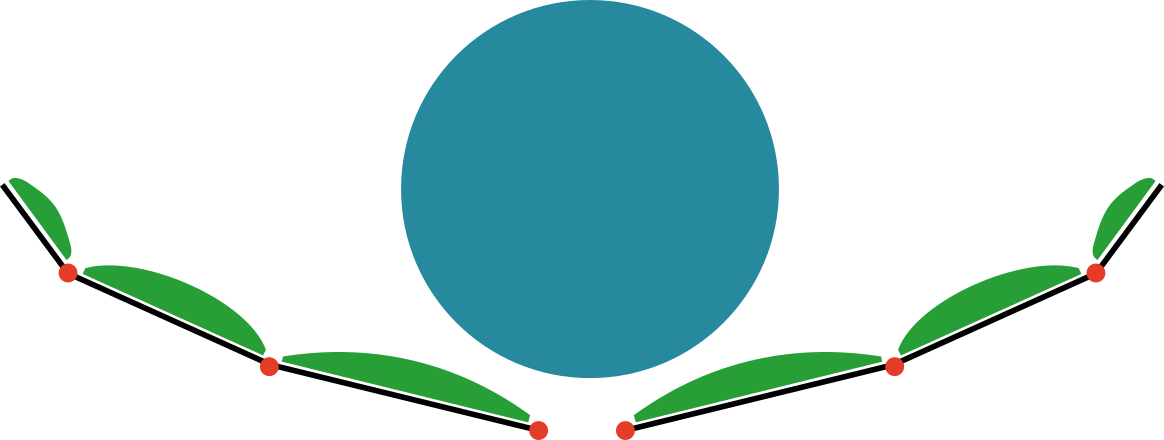
\includegraphics[width=0.7\textwidth]{Images/Underactuaction/FullyOpen.png}
\caption{Fully Open}
        \label{fig:UAFullyOpen}
    \end{subfigure}
    \begin{subfigure}{.45\linewidth}
        \centering
        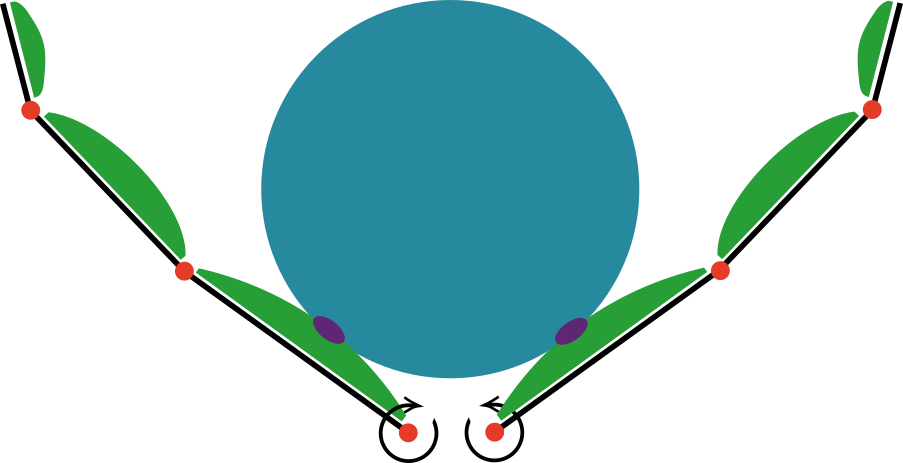
\includegraphics[width=0.7\textwidth]{Images/Underactuaction/phase1png.png}
%    
\includegraphics[width=.4\textwidth]{Images/placeholder.png}

\caption{Step 1, Bottom phalanx rotates and makes contact}
        \label{fig:UAStep1}
    \end{subfigure}
\begin{subfigure}{.45\linewidth}
        \centering
 %   
\includegraphics[width=.4\textwidth]{Images/placeholder.png}       
    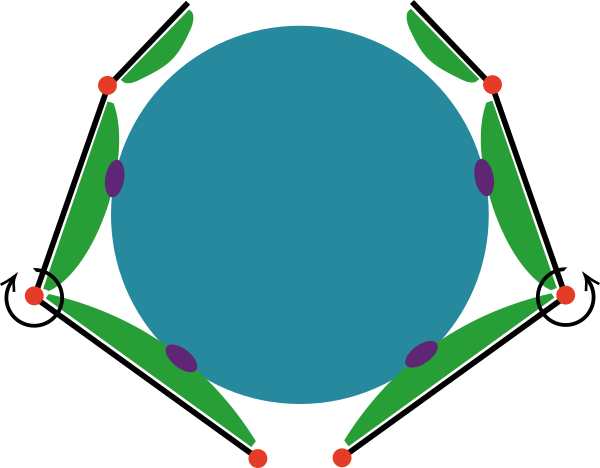
\includegraphics[width=0.7\textwidth]{Images/Underactuaction/phase2.png}

\caption{Step 2, Middle phalanx rotates and makes contact}
        \label{fig:UAStep2}
    \end{subfigure}
    \begin{subfigure}{.45\linewidth}
        \centering
        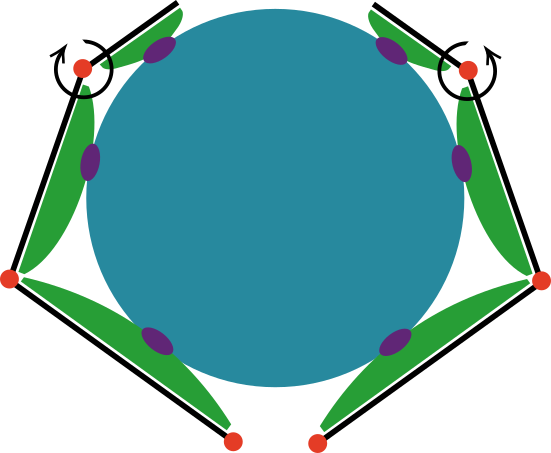
\includegraphics[width=0.7\textwidth]{Images/Underactuaction/FullyClosed.png}
%    
\includegraphics[width=.4\textwidth]{Images/placeholder.png}
\caption{Step 3, Top phalanx rotates and makes contact. Fully Closed}
        \label{fig:UAStep3}
    \end{subfigure}
    \caption{Basic example of underactuation}
    \label{fig:UnderActucation}
\end{figure}




\section{Planning vs Reactive Grasping Strategies}

Literature reflecting on the Amazon Picking Challange (APC) 2015 \cite{Eppner2018} proposes that the development of a robotic system can be described on 4 different spectra. Modularity verus integration, generality vs assumptions, computation versus embodiment and planning versus feedback. It is the last of these which is most relevant when discussing grasping strategies.

In the context of grasping, a fully planning based control strategy adheres strictly to a sense-plan-act structure. Manipulation and grasping is oblivious to sensor stimulus after the sense stage. This approach to grasping requires a static, controlled and structured environment. The opposite is a strategy based wholly on feedback with no high level planning. Instead all actuation is directly caused by sensor stimulus in real time. This type of strategy, while adaptable to changes in the environment, makes it very difficult to complete high level, complex tasks.

%aworld model, leading to verifiable solutions. Feedback from physical interactions, on the other hand, reduces uncertainty and allows to find local solutions without expensive compu- tation. We thus suggest to use planning only when necessary and explore the use of feedback as an alternative when the manipulation task does not require global search."  Feedback is identified as a way to grasp objects which are typically more difficult to grasp. It is identified as something which can be used to combat picking wrong objects, smaller objects, objects which move, the shelf moving. "Manipulation tasks in particular can be gratly simplified by exploiting feedback from contact with the environment""Feedback approaches are particularly useful in the presence of uncertainty, high dimensionality, long time horizons and inaccurate models""Planning would be time-consuming, computationally demanding"

An effective way to examine current state of the art in grasping strategies is to examine approachs taken in robotic competitions. The robotics community often poses challanges and encourages research in particular areas through robotics competitions. Examples of these include RoboCup, RocKIn, and the Amazon Picking Challange (APC). These competitions and the tasks set by them are often used as benchmarks for the performance of different robotic systems and approaches \cite{CompetitionsAsBenchmarks}. The concensis from reflections on these competitions are that although both planning stragtegies, as used by the Delft team in 2016 \cite{Delft}, and reactive strageties, as used by team RBO in 2015, have their strengths, they both won the competition in their respective years, a hybrid control strategy is a more effective solution for robotic gripper \cite{APCObservations}.

\section{Computation}
A common problem which arises in moving object grasping is the high computational overhead associated with a heavy reliance on machine vision and motion planning techniques\cite{KinematicallyOptimal,Eppner2018}. As an example, research conducted by Berthold et al. (2010) \cite{KinematicallyOptimal} used optimised parallel computational loads spread across 32CPU cores in order to perform real-time optimisations for catching a flying ball. Despite advances in computer architectures and software optimisation since that research, the problem of high computational effort remains a significant one. 

Precision is also a major limiting factor for approaches based on only on vision sensors. It is reiterated throughout the literature that "high precision in space and time" is one of the greatest challenges for catching a ball thrown in three dimensional space \cite{RollinJustin}. In that particular example the estimate of the interception position and time need to be accurate within 2cm and 5ms.


\section{Grasping Moving Objects}

Dynamic objects adds another significant challenge to the manipulation problem. Robotic interaction with moving objects has long been a topic of research in robotics\cite{Buhler1989, 1991BallTracking}. Previous research shows robots grasping \cite{ConveyorBeltTracking, ConveyorUnknownObject}, catching \cite{TennisRacket, RollinJustin, DisneyRobot, HandEye, CatchingSoftly}, batting \cite{Muelling2014, Senoo2006} and juggling \cite{JugglingWithKitchenFunnels, Buhler1989, OneHandedJuggling}. These abilities enabled a range of new robotic applications this will be discussed below.

\begin{itemize}
    \item Games and Sports
    
    Much of the research to date which examines how robots could interact with moving objects involve enabling a robot to participate in a sports activities. One of the earliest examples of research in this area is using robots to play ping-pong \cite{Anderson1989}. This area of research has been very active since and there has been continuous improvements have been made \cite{Koc2018}. Other examples of research endowing robots with the ability to play games or sport include Soccer \cite{RoboCupSoccer}, Kendama \cite{Kendama}, Ice Hockey \cite{IceHockey} and Air Hockey \cite{AirHockey}. Both soccer and hockey have been facilitated by Robocup. Robocup is an international robotics competition in which teams of robots compete against each other. Research inspired or guided by these competitions has lead to advancements in robotic design, computer vision, multi-agent systems and many other robotic fields including interaction with dynamic objects \cite{RoboCupSoccer, FuzzyRobocup}. 
    
    \item Human Robot Interaction
    
    The ability to grasp a moving object is also used to as a means of allowing humans to interact with robots. Disney designed a system which could operate in a theme park and could interact which visitors. Identifying contact based human-robot interaction as a potential safety issue, a robot which could play catch was developed \cite{DisneyRobot}. Playing catch as a means to interact with a robot is not a concept unique to Disney. Other research has identified playing catch as a "simple, safe, and fun way" to interact with a robot \cite{JugglingWithKitchenFunnels}.
    
    \item Operating in an unstructured environment
    
    Investigating the autonomous grasping of moving object doesn't always map to a use case where the developed ability can be directly applied. Much of the literature identifies the grasping moving objects as a way to address challenges which are associated with deploying robots in unstructured environments. Grasping or otherwise interacting with a moving objects is a complex task which has demanding temporal and spacial constraints \cite{Anderson1989, EarlyAnticipation}. Investigating the grasping of moving objects has enabled the exploration of novel trajectory generators \cite{Senoo2006, Lampariello2011}, sensor-based reactive motion \cite{Senoo2006} and energy optimisation \cite{Lampariello2011} to name a few . These are explored in the context of a ball catching use case but can be applied more generally to enable robots to operate in unstructured environments 
\end{itemize}


Since this research focuses on grasping we can categorise the most relevant examples to date into four different levels of increasing difficulty based on the behaviour of the target object.

\begin{enumerate}
    \item Regular Object, controlled trajectory (Figure \ref{fig:ConvBelt})
    \item Irregular object, controlled trajectory (Figure \ref{fig:MilkConvy})
    \item Regular object, uncontrolled trajectory (Figure \ref{fig:DisneyBot})
    \item Irregular object, uncontrolled trajectory (Figure \ref{fig:TennisRacket}) 
\end{enumerate}

\begin{figure}
    \centering
    \begin{subfigure}{.4\linewidth}
        \centering
        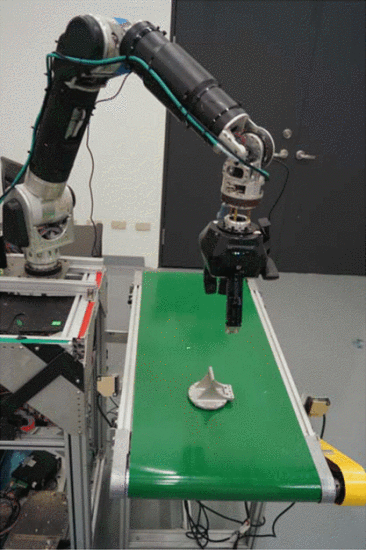
\includegraphics[width=.8\textwidth]{Images/ConveyorBelt.png}
%    
\includegraphics[width=.4\textwidth]{Images/placeholder.png}
        \caption[Category 1: Machined Part on a Conveyor Belt]{Category 1: Machined Part on a Conveyor Belt \cite{ConveyorBeltTracking}}
        \label{fig:ConvBelt}
    \end{subfigure}
    \begin{subfigure}{.5\linewidth}
        \centering
        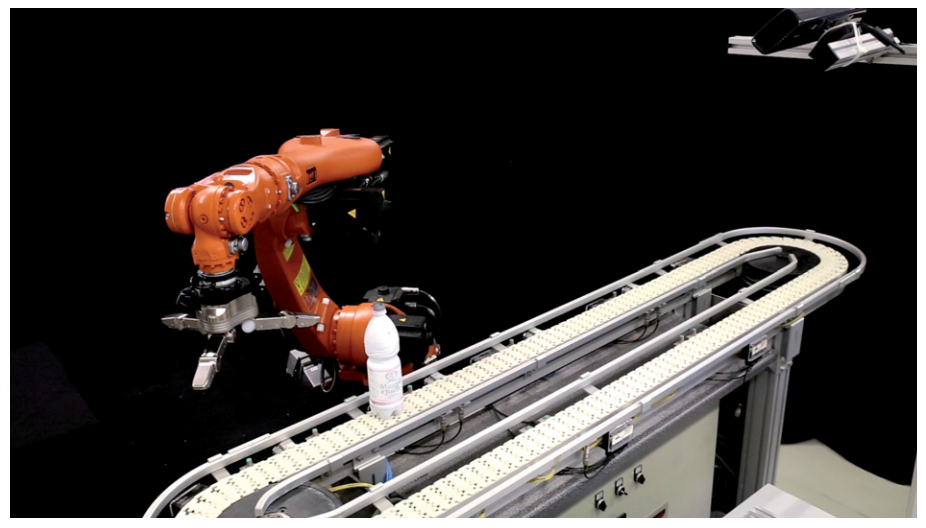
\includegraphics[width=.8\textwidth]{Images/ConveyorUnknown.png}
%    
\includegraphics[width=.4\textwidth]{Images/placeholder.png}
       \caption[Category 2: Grasping an Unknown Object on a Conveyor Belt]{Category 2: Grasping an Unknown Object on a Conveyor Belt \cite{ConveyorUnknownObject}}
        \label{fig:MilkConvy}
    \end{subfigure}
    \begin{subfigure}{.4\linewidth}
        \centering
        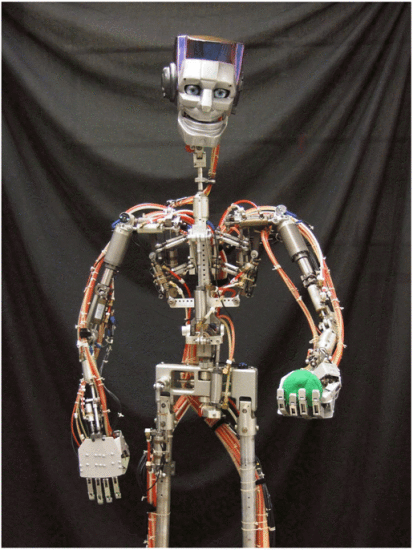
\includegraphics[width=.8\textwidth]{Images/Disney.png}
%    
\includegraphics[width=.4\textwidth]{Images/placeholder.png}
        \caption[Category 3: Theme Park Juggling Robot by Disney]{Category 3: Theme Park Juggling Robot by Disney \cite{DisneyRobot}}
        \label{fig:DisneyBot}
    \end{subfigure}
    \begin{subfigure}{.5\linewidth}
        \centering
    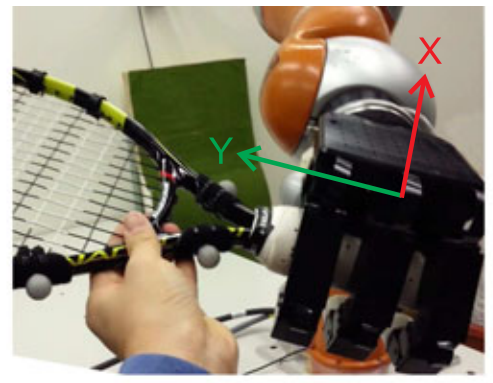
\includegraphics[width=.8\textwidth]{Images/CatchingObjectInFlight.png}
        \caption[Category 4: Catching a Thrown Tennis Racket]{Category 4: Catching a Thrown Tennis Racket \cite{DisneyRobot}}
        \label{fig:TennisRacket}
    \end{subfigure}
\end{figure}

Grasping or otherwise interacting with a moving object is something that is often applied in automation applications to increase the efficiency and throughput of automated process. Potential situations where it might be necessary to grasp a moving object include visual quality checks of finished parts or, as shown in figure \ref{fig:SortingChewingGum}, sorting and/or regularising the orientation of objects on an assembly line. For this reason, a common application where a robot may be required to grasp a moving object is when the object is on a conveyor belt \cite{ConveyorBeltTracking, FingertipEmitterReceiverMovingObjectII,FingertipEmitterReceiverMovingObject}; there are even examples of tactile sensing being used to inform a grasp during manipulation of an object on a conveyor belt \cite{ConveyorUnknownObject}. The context in which these robots are operating is very different from the unstructured scenarios of everyday life; objects are moving at a relatively slow, constant, speed, making them much easier to localise, predict their behaviour, and subsequently grasp them.

\begin{figure}
    \centering
    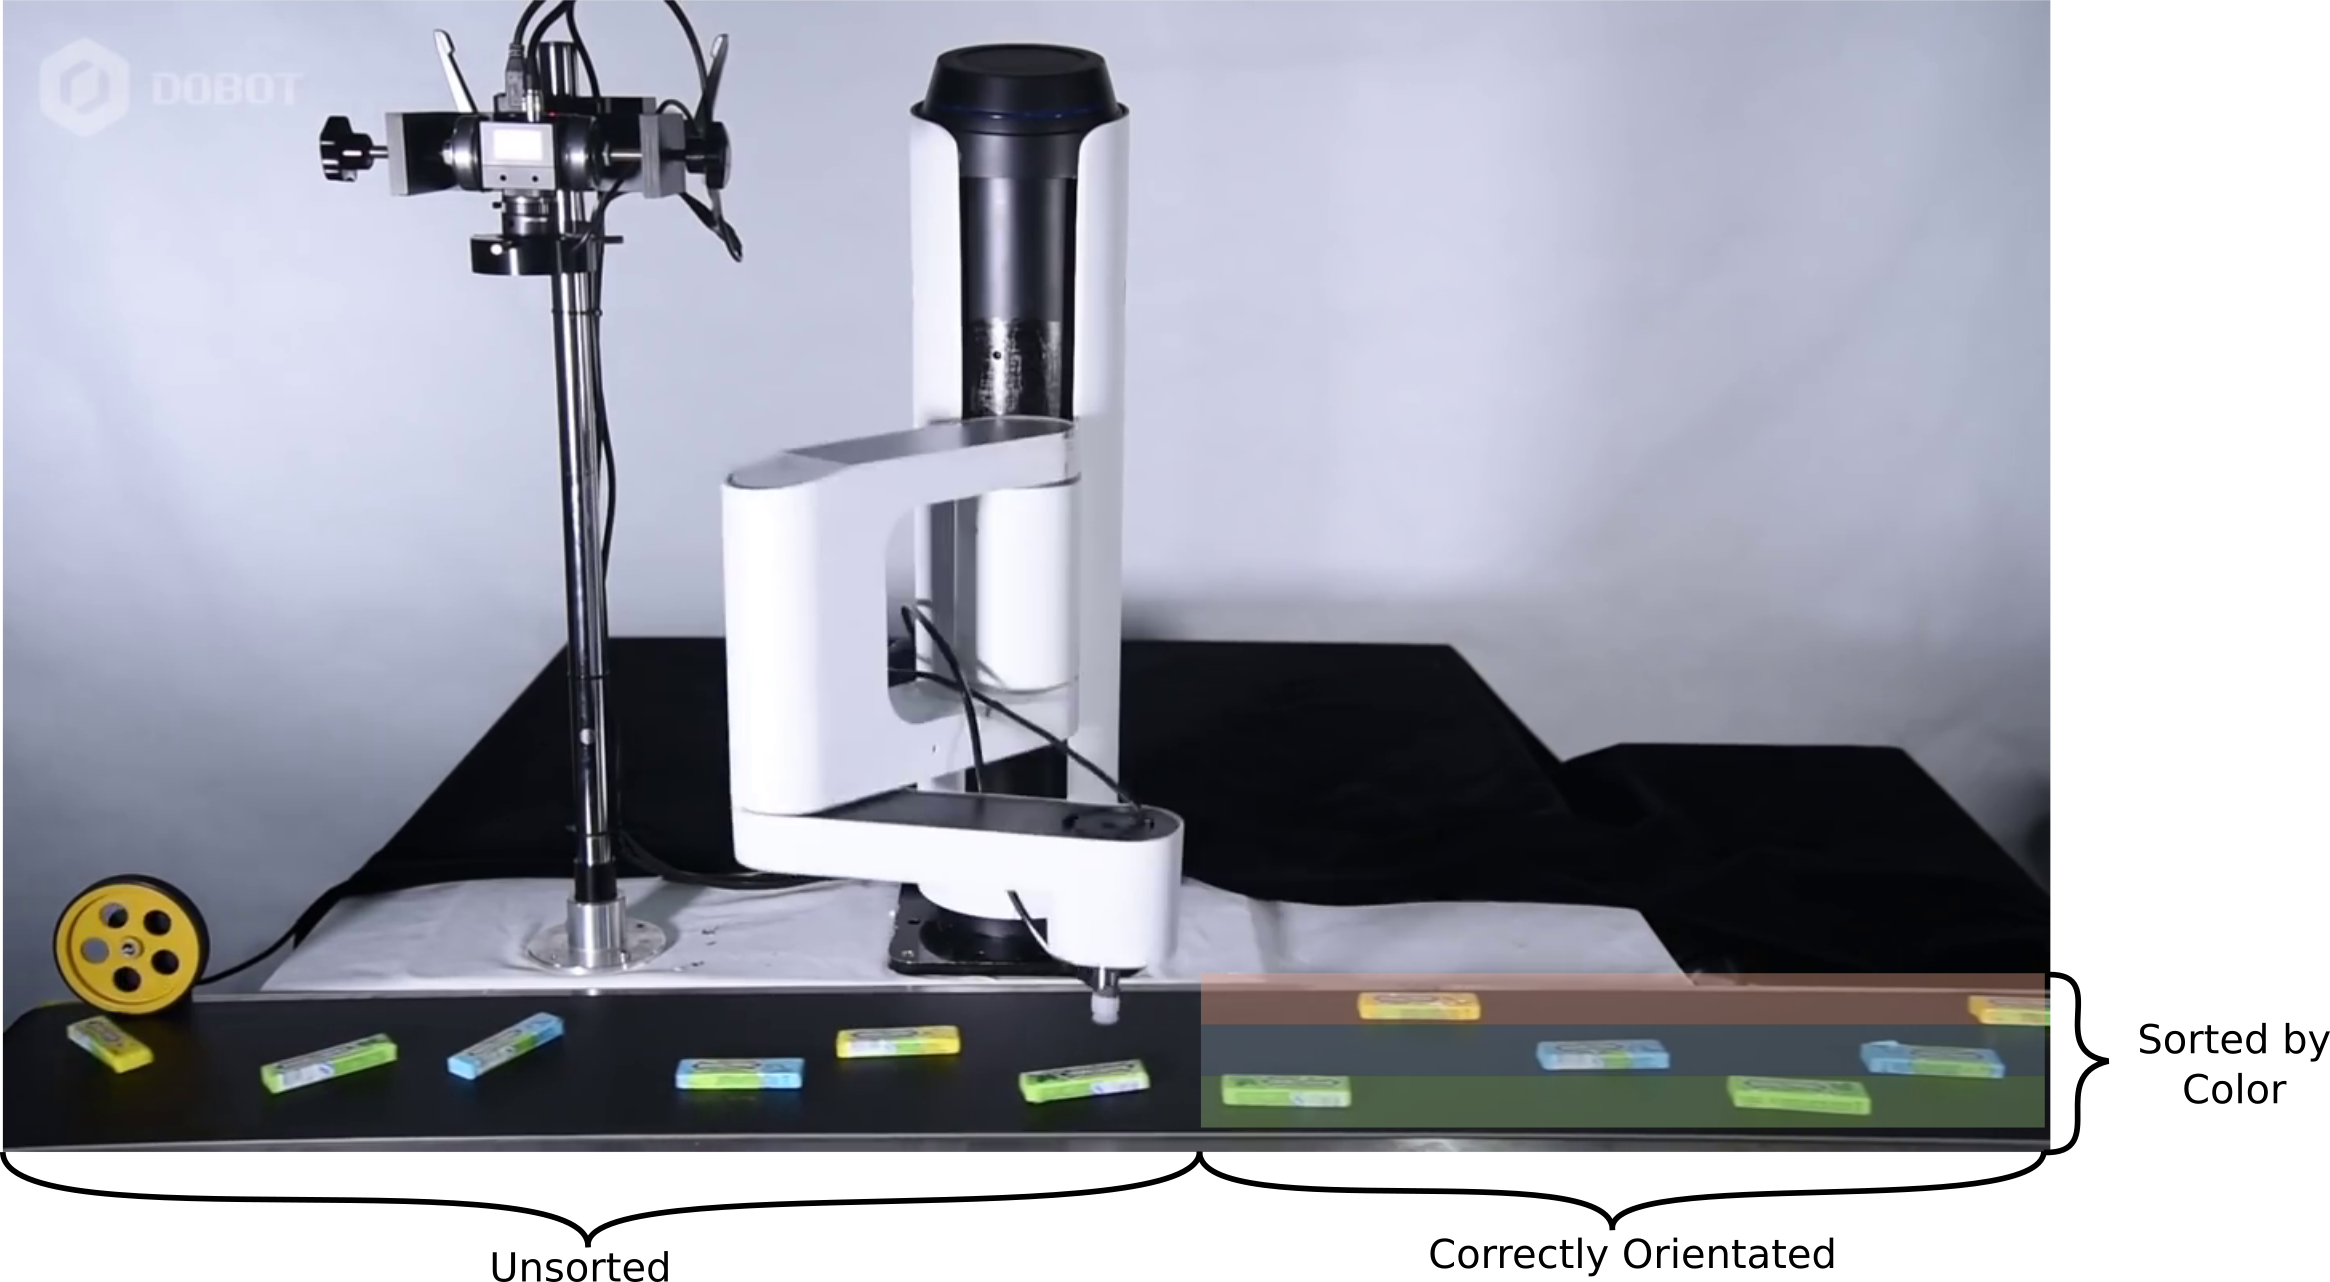
\includegraphics[width=.8\textwidth]{Images/Sorting.png}
%    
\includegraphics[width=.4\textwidth]{Images/placeholder.png}
    \caption{Dobot M1, soring and orientating chewing gum}
    \label{fig:SortingChewingGum}
\end{figure}

The grasping task becomes more complex with the complexity of the object geometry. When grasping simple cuboids, such as the chewing gum example, the grasping task is relatively simple. This is more difficult when grasping irregular objects such as bottles, cups and pitchers \cite{ConveyorUnknownObject}. In this particular example tactile sensing is used to inform the grasp however the object is on a conveyor belt and its speed is therefore known and constant. Although more challenging than grasping static objects, grasping problems on a conveyor belt can effectively be simplified to grasping a static object by first matching the velocity of the target object in the axis of movement during the grasp \cite{FingertipEmitterReceiverMovingObjectII,FingertipEmitterReceiverMovingObject}. 

When the movement of the object is less controlled the problem complexity increases again. An example of this which has long been an active research area is the catching of spherical objects which have been thrown through the air at the robot \cite{1991BallTracking}. Spherical objects are common in research concerned with the grasping of moving objects in non-structured domains \cite{DisneyRobot,RollinJustin,EarlyAnticipation}. These objects are well suited to moving object grasping as they present the same grasping problem regardless of orientation. 

An example of this, already mentioned above, is the Disney created robot, designed to work in theme parks. Developed as an attraction for park visitors, who could interact with the robot without being physically close or needing to contact the robot which was considered a safety concern. The robot could catch a ball which was thrown to it and would throw the ball back to the user. The approach taken massively simplified the grasping motion of the fingers by using a soft ball and foam extension to the gripper to increase the area of the hand and therefore the interception area which would result in a successful grasp. Rollin Justin has also been applied to a ball catching problem, in this case the robot could catch two balls that were thrown simultaneously. In order to achieve this a high number of degrees of freedom were needed, not just the arms but the torso and the mobile platform itself. Both of these examples focus solely on vision sensors to locate and track the object. An estimation of an interception position and time was then used to move the gripper into the correct position and orientation. Neither example examined the closing motion of the gripper, opting instead to close the fingers when the estimation suggested the target object was in the optimum location. 

The final level of complexity for which examples can be seen in the research are successful attempts to dynamically grasp objects with complex geometries, these include tennis rackets and water bottles \cite{TennisRacket}. In this example the additional complexity is addressed by employing more advanced (local and distributed) vision sensing, deep learning and a programming by demonstration approach \cite{TennisRacket}.

In all these examples, the focus of the research is on the vision system, which predicts an intercept position and time, or the mechanical system and achieving the intercept position within a short time window. They have largely ignored (or simplified) the interaction between the gripper and object. For example in the Kendama study \cite{Kendama}, the robot has a bespoke end-effector for catching the ball without the need for a grasp, the Disney gripper \cite{DisneyRobot} uses a foam rim to simplify catching. A more comprehensive review of how research to date has simplified the grasping motion is outlined in section \ref{GraspingMotion}.

\subsection{Grasping Motion}\label{GraspingMotion}

The area of interest for this project is the grasping motion itself, grasping motion in this context specifically refers to the motion of the gripper and fingers as they interact with the object. Many of the examples of the autonomous grasping of moving objects given above focus on either the calculation of an appropriate interception position and time or the ability of the robot to move into position sufficiently quickly. There is a lack of research about, and therefore understanding of, the optimum grasping motion since typically this part of the problem is simplified to a rapid closing of the fingers \cite{RollinJustin, KinematicallyOptimal} or by using solutions like kitchen funnels \cite{EarlyAnticipation}, and foam \cite{DisneyRobot} to remove the need for a robust grasp. Table \ref{Simplifications} shows a history of research concerned with the grasping of moving objects. It demonstrates how the complexity of the motion of the gripper itself if generally abstracted so as to investigate other parameters.

\begin{table}[ht]
\begin{tabular}{|l|l|l|l|l|}
\hline
\textbf{Robot}& \textbf{Year} & \textbf{End Effector} & \textbf{Dimensions} & \textbf{ref} \\ \hline

\begin{tabular}[c]{@{}l@{}}Four DOF, Cable\\ Driven Arm\end{tabular}& 1991 & \begin{tabular}[c]{@{}l@{}}None, Tracking\\ Only \end{tabular} & N/A & \cite{1991BallTracking} \\ \hline

DLR robotic arm & 2001 & "Net" & \diameter160mm & \cite{2001OffTheShelf} \\ \hline

Humanoid Robot & 2002 & \begin{tabular}[c]{@{}l@{}}Kitchen Funnels and \\ Baseball Glove \end{tabular} & Unknown & \cite{JugglingWithKitchenFunnels} \\ \hline

Saika Robto & 2002 & "Cooking Basket" & \diameter120mm & \cite{Saika} \\ \hline

\begin{tabular}[c]{@{}l@{}}Whole Arm\\ Manipulator \end{tabular} & 2005 & \begin{tabular}[c]{@{}l@{}}"{[}T{]}hree DOF\\ end effector"\end{tabular} & Unknown & \cite{HandEye} \\ \hline

6-DOF COTS Arm & 2007 & Cardboard Basket & \diameter 140mm & \cite{COTS} \\ \hline

DLR-LWR-III arm & 2010 & DLR-Hand-II & Unknown & \cite{KinematicallyOptimal} \\ \hline

Rollin' Justin & 2011 & \begin{tabular}[c]{@{}l@{}}12 DOF, DLR-Hand-II \\ see Fig. \ref{fig:RollingJustinHand} \end{tabular} & $ \approx  140mm^2 $ & \cite{RollinJustin} \\ \hline

\begin{tabular}[c]{@{}l@{}}Sky, a Disney \\ Humanoid Robot\end{tabular} & 2012 & \begin{tabular}[c]{@{}l@{}}Humanoid Gripper, "augmented\\ ...{[}by{]} a foam rim to provide a \\ more cup-like shape suitable for\\ catching" see Fig. \ref{fig:DisneyFoam} \end{tabular} & \begin{tabular}[c]{@{}l@{}} $ 100mm^2 $ \\ $ + foam $ \end{tabular} & \cite{DisneyRobot} \\ \hline

Kuka LWR4+ & 2014 & 16-DOF Allegro Hand & Unknown & \cite{TennisRacket} \\ \hline

\end{tabular}
\caption{End effectors used to grasp moving objects}
\label{Simplifications}
\end{table}

\begin{figure}
    \centering
    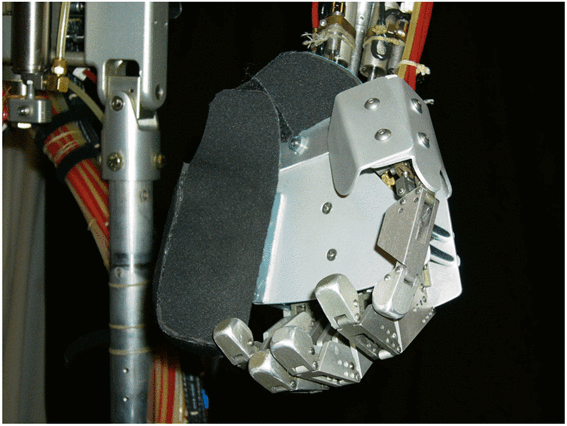
\includegraphics[width=.4\textwidth]{Images/DisneyFoam.png}
%    
\includegraphics[width=.4\textwidth]{Images/placeholder.png}
    \caption{Foam Augmentation to the Disney hand to facilitate grasping \cite{DisneyRobot}}
    \label{fig:DisneyFoam}
\end{figure}
\begin{figure}
    \centering
    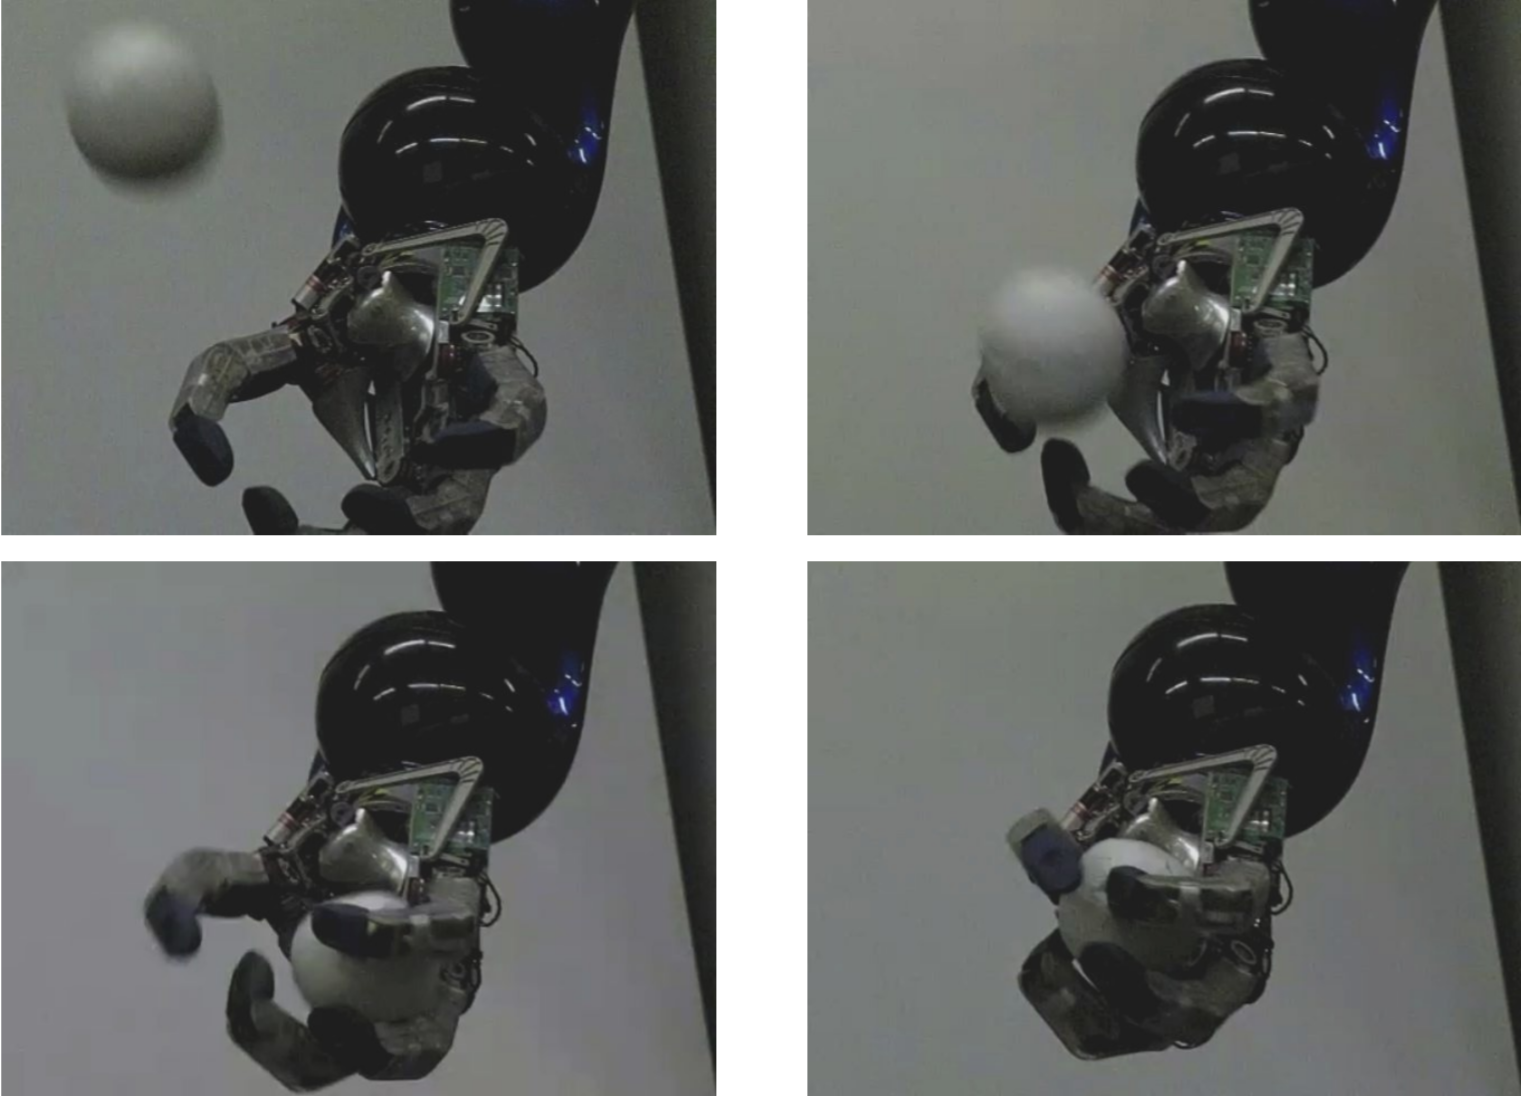
\includegraphics[width=.4\textwidth]{Images/RollingJustinHand.png}
%    
\includegraphics[width=.4\textwidth]{Images/placeholder.png}
    \caption{DLR-II Hand used on Rollin Justin \cite{RollinJustin}}
    \label{fig:RollingJustinHand}
\end{figure}


\section{Research Contribution}
In a survey conducted on competitors in the 2015 Amazon Picking Challenge \cite{APCObservations}, the introduction of reactive control was was the dominant response from participants when ask to reflect on what changes they would make to their system. In the same survey 84\% of respondents agreed with the statement that "Perception needs to be better integrated with motion planning" and 68\% agree that "Motion planning needs to be better integrated with reactive planning". This study concluded that "the use of reactive control to compensate for inaccurate sensing and actuation of an underlying deliberative architecture appears to be powerful". This sentiment is echoed throughout the literature, sensory feedback is said to be a necessity in order to robustly perform high speed tasks \cite{Senoo2006}. Despite this apparent agreement amongst researchers on the need for reactive control based on sensory input this review of the existing literature has found that the contribution of sensing in grasping moving objects is a under-explored area, this project aims to tackle this.




